\usetikzlibrary{plotmarks}

\begin{figure}[htbp]
\centering
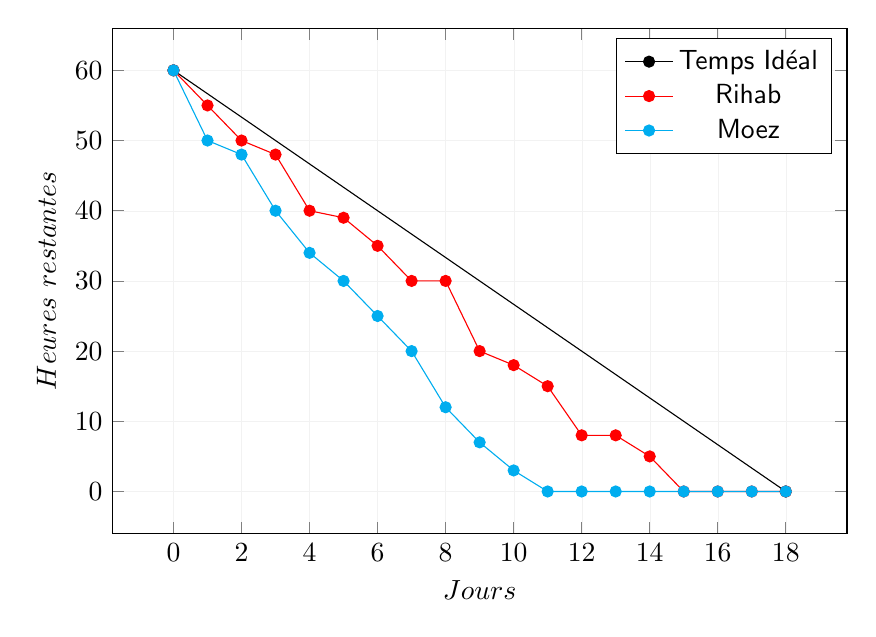
\begin{tikzpicture}[y=.2cm, x=.7cm,font=\sffamily]
\begin{axis}[
xlabel=$Jours$,
ylabel=$Heures\ restantes$,
grid=both,
grid style={line width=.1pt, draw=gray!10},
width=0.9\textwidth,
height=8cm,
%major grid style={line width=.2pt,draw=gray!50},
]
\addplot[color=black,mark=*] coordinates {
        (0,60)
        (18,0)
    };
    \addlegendentry{Temps Idéal}

    \addplot[mark=*,red] plot coordinates {
        (0, 60)
        (1, 55)
        (2, 50)
        (3, 48)
        (4, 40)
        (5, 39)
        (6, 35)
        (7, 30)
        (8, 30)
        (9, 20)
        (10, 18)
        (11, 15)
        (12, 8)
        (13, 8)
        (14, 5)
        (15, 0)
        (16, 0)
        (17, 0)
        (18, 0)
       
    };
    \addlegendentry{Rihab}
      \addplot[mark=*,cyan] plot coordinates {
        (0, 60)
        (1, 50)
        (2, 48)
        (3, 40)
        (4, 34)
        (5, 30)
        (6, 25)
        (7, 20)
        (8, 12)
        (9, 7)
        (10, 3)
        (11, 0)
        (12, 0)
        (13, 0)
        (14, 0)
        (15, 0)
        (16, 0)
        (17, 0)
        (18, 0)
       
    };
    \addlegendentry{Moez}
\end{axis}
\end{tikzpicture}
\caption{Graphique d'avancement - Itération 1}
\end{figure}
